\documentclass{beamer}
\usepackage[utf8]{inputenc}
\usepackage{color}
\usepackage{multirow}
\usepackage{mathbbol}
\usepackage{amssymb}
\newcommand{\mybinom}[3][0.8]{\scalebox{#1}{$\dbinom{#2}{#3}$}}
\newcommand\scalemath[2]{\scalebox{#1}{\mbox{\ensuremath{\displaystyle #2}}}}

\setbeamercovered{transparent}
\setbeamertemplate{itemize items}[circle]

% \logo{\includegraphics[height=1.0cm]{ATM.png}}
\setbeamertemplate{sidebar right}{}
\setbeamertemplate{footline}{
\hfill\usebeamertemplate***{navigation symbols}
\hspace{1cm}\insertframenumber{}/\inserttotalframenumber}


\title[About Beamer] %optional
{Fundamental Limits of Coded Caching: From Uncoded Prefetching to Coded Prefetching}

\author{Kai Zhang and Chao Tian}

\institute{Texas A\&M University}

\date{ISIT 2018}


\begin{document}

\frame{\titlepage}

% ========  1  =================
\begin{frame}
\frametitle{Caching and Its Applications}

  A natural data management strategy
  \begin{itemize}
  \item Prefetching data to local/fast memory space;
  \item<2-> Single user setting, e.g. RAM in computers, on-CPU caches;
  \item<3> Multiple user setting, e.g. networked system.
  \end{itemize}
  
 % \vspace{0.5cm}
  
  \begin{figure}
  \centering
   	 \includegraphics<1>[height=4cm]{networkCaching0.jpg}
 	\includegraphics<2>[height=4cm]{cacheonRAM.pdf}
  	\includegraphics<3>[height=4cm]{contentcache}%{networkCaching.jpg}
\end{figure}
\end{frame}

% ========  2  =================
\begin{frame}
\frametitle{An Information-theoretic Formulation}
  Proposed by Maddah-Ali \& Niesen\footnotemark
  \begin{itemize}
  \item $N$ files of same size, $K$ users, each with local cache of size $M$;
  \item<2>Prefetching phase: users fill cache before knowing requests;
  \item<2> Delivery phase: server multicasts information.
  \end{itemize}
  \vspace{0.3cm}
  \centering
  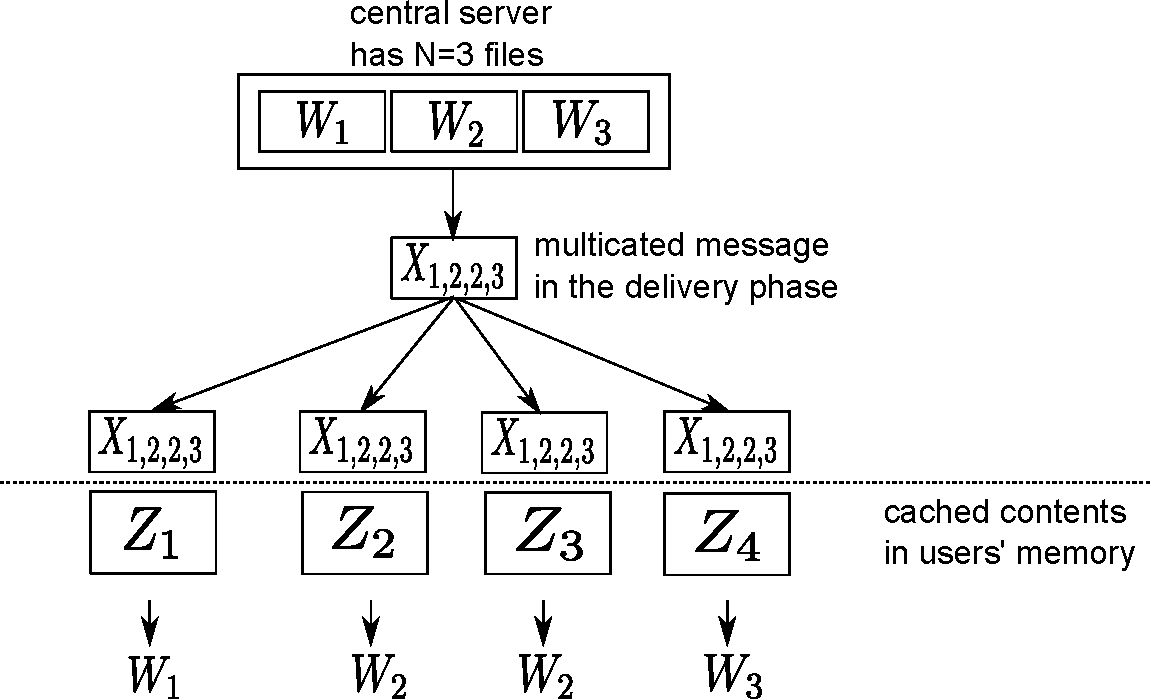
\includegraphics[width=0.65\textwidth]{system_diag}
%  \vspace{0.3cm}
%  \includegraphics[scale = 0.27]{cacheNetwork.png}
  \footnotetext[1]{\tiny Maddah-Ali  \& Niesen, \lq\lq{}Fundamental limits of caching,\rq\rq{} TIT-14.}
\end{frame}

% ========  3  =================
\begin{frame}
\frametitle{Existing Schemes Using Uncoded Prefetching}
  Maddah-Ali-Niesen scheme: uncoded prefetching
  \begin{itemize}
  \item Partition each file into $\binom{K}{t}$ segments;
  \item Each user allocated $\binom{K-1}{t-1}$ uncoded segments.
  \end{itemize}
  \vspace{1.5cm}
  
 \fbox{
 \begin{minipage}{0.99\textwidth}
  \onslide<2>{Example $(N,K) = (3,4), t = 2$:}
  \begin{table}\onslide<2->
  \centering
  \begin{tabular}{|l||l|l|l|l|l|l|l|l|l|}
  \hline
  User 1 & $A_{12}$ & $A_{13}$ & $A_{14}$ & $B_{12}$ & $B_{13}$ & $B_{14}$ & $C_{12}$ & $C_{13}$ & $C_{14}$ \\ \hline
  User 2 & $A_{12}$ & $A_{23}$ & $A_{24}$ & $B_{12}$& $B_{23}$ & $B_{24}$ & $C_{12}$ & $C_{23}$ & $C_{24}$ \\ \hline
  User 3 & $A_{13}$ & $A_{23}$ & $A_{34}$ & $B_{13}$ & $B_{23}$ & $B_{34}$ & $C_{13}$ & $C_{23}$ & $C_{34}$ \\ \hline
  User 4 & $A_{14}$ & $A_{24}$ & $A_{34}$ & $B_{14}$ & $B_{24}$ & $B_{34}$ & $C_{14}$ & $C_{24}$ & $C_{34}$\\ \hline
  \end{tabular}
  \end{table}
  \end{minipage}}
\end{frame}


% ========  4  =================
\begin{frame}
\frametitle{Existing Schemes Using Uncoded Prefetching}
Delivery phase: multicast information to fulfill all requests
\begin{itemize}
\item Enumerate all $(t+1)$-user set $\mathcal{B}$;
\item<2-> Each set $\mathcal{B}$ determines a transmission;
\item<3-> Each transmission contains only one missing symbol for a user.
\end{itemize}
\vspace{0.2cm}
\fbox{
\begin{minipage}{0.95\textwidth}
\onslide<4->{Example $(N,K) = (3,4), t = 2$, demand $(A,A,B,C)$}
\begin{align*}
& \onslide<4->{\mathcal{B}=\{1,2,3\}: A_{23} +A_{13}+B_{12};} \\
& \onslide<4->{\mathcal{B}=\{1,2,4\}: A_{24} +A_{14}+C_{12};} \\
& \onslide<4->{\mathcal{B}=\{1,3,4\}: A_{34} +B_{14}+C_{13};} \\
& \onslide<4->{\mathcal{B}=\{2,3,4\}: A_{34} +B_{24}+C_{23}.}
\end{align*}
\end{minipage}
}

\vspace{0.6cm}
\onslide<5>{Yu's scheme\footnotemark[1] improved it by removing linearly redundant terms for some $(N,K)$ values.}
\onslide<5>{\footnotetext[1]{\tiny Yu et al. \lq\lq{}The exact rate-memory tradeoff for caching with uncoded prefetching,\rq\rq{} TIT-17.}}
\end{frame}
%
%% ========  5  =================
%\begin{frame}
%\frametitle{Existing Schemes Using Uncoded Prefetching}
%For demand $(A,A,B,C)$, user 1 has:
%\begin{table}[]
%\centering
%\begin{tabular}{|l||l|l|l|l|l|l|l|l|l|}
%\hline
%User 1 & $A_{12}$ & $\alert<1->{A_{13}}$ & \alert<2->{$A_{14}$} & $\alert<1->{B_{12}}$ & $B_{13}$ & $\alert<3->{B_{14}}$ & \alert<2->{$C_{12}$} & $\alert<3->{C_{13}}$  & $C_{14}$ \\ \hline
%\end{tabular}
%\end{table}
%Transmissions are 
%\begin{align*}
%& \textcolor<1->{blue}{A_{23}} +\alert<1->{A_{13}}+\alert<1->{B_{12}}, \quad  \textcolor<2->{blue}{A_{24}} +\alert<2->{A_{14}}+\alert<2->{C_{12}} \\
%& \textcolor<3->{blue}{A_{34}} +\alert<3->{B_{14}}+\alert<3->{C_{13}} ,\quad  A_{34} +B_{24}+C_{23}
%\end{align*}
%
%\begin{itemize}
%	\item<only@1> Step 1: use \alert{$A_{13}$} and \alert{$B_{12}$} to decode \textcolor{blue}{$A_{23}$};
%	\item<only@2>  Step 2: use \alert{$A_{14}$} and \alert{$C_{12}$} to decode \textcolor{blue}{$A_{24}$}
%	\item<only@3>  Step 3: use \alert{$B_{14}$} and \alert{$C_{13}$} to decode \textcolor{blue}{$A_{34}$}.
%\end{itemize}



%\end{frame}

% ========  6 =================
\begin{frame}
\frametitle{Existing Schemes Using Coded Prefetching}
T. and Chen\footnotemark[1] proposed a scheme using coded prefetching
\footnotetext[1]{\tiny T.\&Chen, \lq\lq{}Caching and delivery via interference elimination,\rq\rq{}  TIT-18.}
\begin{itemize}
\item Partition each file into $\binom{K}{t}$ segments;
\pause
\item User encodes allocated file segments using rank metric code;
\item The parity symbols are stored.
\end{itemize}
\pause
Delivery phase uses MDS code
\begin{itemize}
	\item Cached contents $\perp$ delivered transmissions; 
	\item Each transmission contains segments from only one file.
\end{itemize}

\vspace{10pt}
\pause
\fbox{
\begin{minipage}{0.95\textwidth}
Example: $(N,K)=(3,4)$, demand = (A,A,B,C), transmits:
\begin{equation*}
A_{34}, \; {B_{12}}, \; B_{14}, \; B_{24}, \; C_{12},\; C_{13}, \; C_{23}, \; {A_{13}}+{A_{23}}, \;  {A_{14}}+{A_{24}}
\end{equation*}
$A_{14}+A_{24}$: needed by users 1\&2; help resolve symbols at user 4.
\end{minipage}
}
%\begin{itemize}
%\item<4> $B_{12}$: required content for user 3; help resolve symbols at users 1 and 2.
%\end{itemize}
%\vspace{10pt}
%\onslide<4>{Example $(N,K) = (3,4), t = 2$, user 1 stores}
%\begin{equation*}
%\scalemath{0.8}{\onslide<4>{\begin{pmatrix}
%    \times   & \times  & \times  & \times &\times   & \times  & \times  & \times & \times \\
%    \times   & \times  & \times  & \times &\times   & \times  & \times  & \times & \times \\
%   \times   & \times  & \times  & \times &\times   & \times  & \times  & \times & \times \\
%    \times   & \times  & \times  & \times &\times   & \times  & \times  & \times & \times \\
%    \times   & \times  & \times  & \times &\times   & \times  & \times  & \times & \times
%\end{pmatrix}_{(5 \times 9)}
%\cdot 
%\begin{pmatrix}
%	A_{12} \\
%	A _{13} \\
%	A_{14} \\
%	B_{12} \\
%	B_{13} \\
%	B_{14} \\
%	C_{12} \\
%	C_{13} \\
%	C_{14}
%	\end{pmatrix}}
%	}
%\end{equation*}

\end{frame}


%% ========  7 =================
%\begin{frame}
%\frametitle{Existing Schemes Using Coded Prefetching}
%Delivery phase uses MDS code
%\begin{itemize}
%	\item Cached contents $\perp$ delivered transmissions; 
%	\item<2-> Each transmission contains segments from only one file.
%\end{itemize}
%\vspace{10pt}
%\onslide<3->Example: $(N,K)=(3,4), t=2$, demand = (A,A,B,C), transmits:
%\begin{equation*}
%A_{34}, \; \textcolor<4>{blue}{B_{12}}, \; B_{14}, \; B_{24}, \; C_{12},\; C_{13}, \; C_{23}, \; \textcolor<4>{red}{A_{13}}+\textcolor<4>{blue}{A_{23}}, \;  \textcolor<4>{red}{A_{14}}+\textcolor<4>{blue}{A_{24}}
%\end{equation*}
%\begin{itemize}
%\item<4> $B_{12}$: required content for user 3; help resolve symbols at users 1 and 2.
%\end{itemize}
%\end{frame}
%
%% ========  7 =================
%\begin{frame}
%\frametitle{Existing Schemes Using Coded Prefetching}
%Delivery phase uses MDS code
%\begin{itemize}
%	\item Cached contents $\perp$ delivered transmissions; 
%	\item Each transmission contains segments from only one file.
%\end{itemize}
%\vspace{10pt}
%Example: $(N,K)=(3,4), t=2$, demand = (A,A,B,C), transmits:
%\begin{equation*}
%A_{34}, \; B_{12}, \; B_{14}, \; B_{24}, \; C_{12},\; C_{13}, \; C_{23}, \; \textcolor<1>{red}{A_{13}}+\textcolor<1>{blue}{A_{23}}, \;  \textcolor<1>{red}{A_{14}}+\textcolor<1>{blue}{A_{24}}
%\end{equation*}
%\begin{itemize}
%\item $A_{14}+A_{24}$: required content for users 1 and 2; help resolve symbols at user 4.
%\end{itemize}
%\end{frame}

% ========  8 =================
%\begin{frame}
%\frametitle{Existing Schemes Using Coded Prefetching}
%Transmissions are 
%\begin{align*}
%A_{34}, \;  \textcolor<1->{blue}{B_{12}, \; B_{14}}, \; B_{24}, \; \textcolor<1->{blue}{C_{12},\; C_{13}}, \; C_{23}, \; A_{13}+ A_{23}, \; A_{14}+A_{24}.
%\end{align*}
%
%\pause
%
%User 1 decodes:
%\begin{itemize}
%\item Step 1: collect \textcolor{blue}{$B_{12}, B_{14},C_{12},C_{13}$} to decode all coded symbols in cache;
%\end{itemize}
%\begin{align*}\onslide<2>
%& \scalemath{0.8}{\begin{pmatrix}
%    \times   & \times  & \times  & \times &\times   & \times  & \times  & \times & \times \\
%    \times   & \times  & \times  & \times &\times   & \times  & \times  & \times & \times \\
%   \times   & \times  & \times  & \times &\times   & \times  & \times  & \times & \times \\
%    \times   & \times  & \times  & \times &\times   & \times  & \times  & \times & \times \\
%    \times   & \times  & \times  & \times &\times   & \times  & \times  & \times & \times \\
%               &           &          &  \textcolor{blue}{\times} &         &         &         &           &       \\
%                   &            &            &           &            & \textcolor{blue}{\times}  &            &   &   \\
%                    &            &            &           &            &            & \textcolor{blue}{\times}  &   &   \\
%                         &            &            &           &            &            &            & \textcolor{blue}{\times} &          
%\end{pmatrix}
%\cdot \begin{pmatrix}
%A_{12}\\
% A_{13}\\
% A_{14}\\
%  B_{12}\\
%   B_{13}\\
%    B_{14}\\
%     C_{12}\\
%      C_{13}\\
%       C_{14}
%       \end{pmatrix}}
%\end{align*}
%\end{frame}
%
%% ========  8.1 =================
%\begin{frame}
%\frametitle{Existing Schemes Using Coded Prefetching}
%Transmissions are 
%\begin{equation*}
%A_{34}, \;  B_{12}, \; B_{14}, \; B_{24}, \; C_{12},\; C_{13}, \; C_{23}, \; \textcolor<1>{red}{A_{13}}+\textcolor<1>{blue}{A_{23}}, \; \textcolor<1>{red}{A_{14}}+\textcolor<1>{blue}{A_{24}}.
%\end{equation*}
%
%\pause
%\vspace{0.5cm}
%
%User 1 now has:
%\begin{table}
%\centering
%\begin{tabular}{|l||l|l|l|l|l|l|l|l|l|}
%\hline
%User 1 & $A_{12}$ & $\textcolor{red}{A_{13}}$ & $\textcolor{red}{A_{14}}$ & $B_{12}$ & $B_{13}$ & $B_{14}$ & $C_{12}$ & $C_{13}$ & $C_{14}$ \\ \hline
%\end{tabular}
%\end{table}
%
%User 1 decodes:
%\begin{itemize}
%\item Step 2: use $\textcolor{red}{A_{13}}, \textcolor{red}{A_{14}}$ to decode \textcolor{blue}{$A_{23}, A_{24}$};
%\item Step 3: collect $\textcolor{blue}{A_{34}}$.
%\end{itemize}
%
%
%\end{frame}
%
%% ========  8.2 =================
%\begin{frame}
%\frametitle{Existing Schemes Using Coded Prefetching}
%Transmissions are
%\begin{equation*}
%A_{34}, \;  B_{12}, \; B_{14}, \; B_{24}, \; C_{12},\; C_{13}, \; C_{23}, \; A_{13}+ A_{23}, \; A_{14}+A_{24}.
%\end{equation*}
%\begin{itemize}
%\item Step 3: collect $\textcolor{blue}{A_{34}}$. \\
%\end{itemize}
%User 1 now decodes the entire file A.
%\end{frame}

% ========  9  =================
\begin{frame}
\frametitle{Two Quite Different Schemes}

\begin{columns}
\begin{column}{0.45\textwidth}
Uncode prefetching:  
\begin{itemize}
\item Binary code
\item Simple combinatorics
\item Better at high memory regime
%\item<2,3,4,5> Allows systematic code \& less meta data (code stays the same over time)\smiley
%\item<3,4,5> Optimal tradeoff unknown
%\item<4,5> Some code constructions
%\vspace{1cm}
%\item<5> Preferred in practice? {{\textcolor{green}{\cmark}}}
\end{itemize}
  \end{column}

  \begin{column}{0.5\textwidth}
Coded prefetching:  
\begin{itemize} 
\item Non-binary code
\item MDS and rank metric codes
\item Better at low memory regime
\end{itemize}
  \end{column}

\end{columns}

%\begin{itemize}
%\item Uncoded \textit{vs.} coded prefetching;
%\item Binary \textit{vs.} non-binary code;
%\item Simple combinatorics \textit{vs.} sophisticated coding techniques (rank metric codes);
%\item Performs better at high memory regime \textit{vs.} low memory regime.
%\end{itemize}
\pause
\vspace{1cm}
\centering
\textit{Are there any connections?}
\end{frame}

%% ========  5  =================
%\begin{frame}
%\frametitle{Some Backgrounds}
%\begin{itemize}
%\item Linearized Polynomial:
%A degree-$q^{P-1}$ linearized polynomial in the finite field $\mathbb{F}_{q^m}$
%\begin{equation}
%f(x) = \sum_{i = 1,2,\ldots, P} v_i x^{q^{i-1}}, v_i \in \mathbb{F}_{q^m}
%\end{equation}
%can be uniquely identified from evaluations at any $P$ points $x = \theta_{i} \in \mathbb{F}_{q^m}, i = 1,2,\ldots, P$, that are linearly independent over $\mathbb{F}_q$.
%\end{itemize}
%\end{frame}

% ========  5.1 =================
%\begin{frame}
%\frametitle{Some Backgrounds}
%\begin{block}{Lemma}
%Let $f(x)$ be a degree-$q^{P-1}$ linearized polynomial in $\mathbb{F}_{q^m}$, and $\theta_i \in \mathbb{F}_{q^m}, i = 1,2,\ldots,P_o$, be linearly independent over $\mathbb{F}_q$. Let $G$ be a $P_o \times P$ full rank (rank $P$) matrix with entries in $\mathbb{F}_q$, then $f(x)$ can be  uniquely identified from 
%\begin{equation}
%[f(\theta_1), f(\theta_2), \ldots, f(\theta_{P_o})] \cdot G.
%\end{equation}
%\end{block}

%\setbeamertemplate{itemize items}[circle]
%\begin{itemize}
%\item $(v_1,\ldots, v_P)$ are information symbols to be encoded; $[f(\theta_1),\ldots,f(\theta_{P_o})]$ are coded symbols;
%\item A $(P_o,P)$ MDS code in terms of rank metric.
%\end{itemize}
%\end{frame}

% ========  6 =================
\begin{frame}
\frametitle{A Hidden Connection}
Putting them side-by-side
\begin{itemize}
\item Maddah-Ali Niesen scheme transmits 4 symbols:
\begin{align*}
& A_{23} +A_{13}+B_{12}, \quad  A_{24} +A_{14}+C_{12} \\
& A_{34} +B_{14}+C_{13} ,\quad  A_{34} +B_{24}+C_{23}
\end{align*}
\end{itemize}
\centering
%Separate different files \& remove repeated transmissions, \\
$\Downarrow$
\begin{itemize}
\item Tian-Chen scheme transmits 9 symbols:
\begin{align*}
& A_{23} +A_{13}, \quad B_{12}, \qquad  A_{24} +A_{14}, \quad C_{12} \\
& A_{34}, \;\;\; B_{14}, \quad C_{13}, \qquad  \qquad \;\;\; B_{24}, \quad C_{23}
\end{align*}
\end{itemize}
\pause
\vspace{0.4cm}
\centering
\textcolor{blue}{Question: Will other decomposition give better performance?}
\end{frame}


% ========  6.1 =================
\begin{frame}
\frametitle{Yes! A New Scheme for $(N,K)=(3,4)$}
A partial decomposition scheme $(N,K)=(3,4), t=2$,
%\begin{itemize}
%	\item Choose some transmissions to decompose;
%	\item From those transmissions, choose some files to decompose.
%\end{itemize}
%\vspace{10pt}

\begin{itemize}
	\item Demand (A,A,B,C), transmits
	\begin{align*}
	& A_{23} +A_{13}+B_{12}, \quad  A_{24} +A_{14}+C_{12} \\
	& A_{34}, \;\;\; B_{14}+C_{13} ,\qquad \quad \;\; B_{24}+C_{23}
	\end{align*}
	i.e. only the last two transmissions, file A is decomposed out.
	\item Demand (A,A,B,B), transmits
	\begin{align*}
	& A_{23} +A_{13}+B_{12}, \quad  A_{24} +A_{14}+B_{12} \\
	& A_{34}, \;\;\; B_{14}+B_{13} ,\qquad \quad \;\; B_{24}+B_{23}
	\end{align*}
%	\item Demand (A,A,A,C), transmits
%	\begin{align*}
%	& A_{23} +A_{13}+A_{12}, \quad  A_{24} +A_{14}+C_{12} \\
%	& A_{34}, \;\;\; A_{14}+C_{13} ,\qquad \quad \;\;A_{24}+C_{23}
%	\end{align*}
	\item ....
\end{itemize}
\end{frame}

%% ========  6.2 =================
%\begin{frame}
%\frametitle{A New Scheme}
%Apply this decomposition pattern to all degenerate demands:
%\begin{itemize}
%	\item Demand (A,A,B,B), transmits
%	\begin{align*}
%	& A_{23} +A_{13}+B_{12}, \quad  A_{24} +A_{14}+B_{12} \\
%	& A_{34}, \;\;\; B_{14}+B_{13} ,\qquad \quad \;\; B_{24}+B_{23}
%	\end{align*}
%	\item Demand (A,A,A,C), transmits
%	\begin{align*}
%	& A_{23} +A_{13}+A_{12}, \quad  A_{24} +A_{14}+C_{12} \\
%	& A_{34}, \;\;\; A_{14}+C_{13} ,\qquad \quad \;\;A_{24}+C_{23}
%	\end{align*}
%	\item Demand (A,A,A,A), transmits
%	\begin{align*}
%	& A_{23} +A_{13}+A_{12}, \quad  A_{24} +A_{14}+A_{12} \\
%	& A_{34}, \;\;\; A_{14}+A_{13} ,\qquad \quad \;\;A_{24}+A_{23}
%	\end{align*}
%\end{itemize}
%\end{frame}


% ========  6.3 =================
\begin{frame}
\frametitle{Performance of the New Scheme}
%\begin{figure}[]
\centering{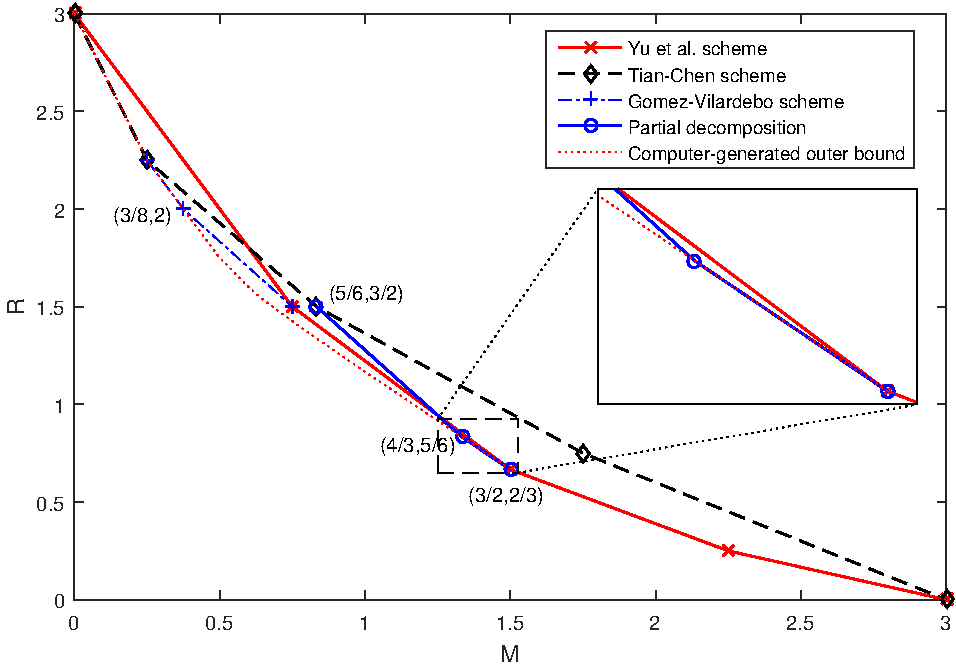
\includegraphics[width=9cm]{plot34.pdf} }

%\end{figure}
\begin{itemize}
\item Produces $(M,R)=(\frac{4}{3},\frac{5}{6})$: a new corner point and optimal.
\end{itemize}

\end{frame}

% ========  7  =================
\begin{frame}
\frametitle{The General Idea}

We know the extremes:
\begin{itemize} 
\item No decomposition: Maddah-Ali-Niesen's (Yu\rq{}s) transmissions;
\item Full decomposition: Tian-Chen's transmissions.
%\item Partial decomposition: only decompose different files.
\end{itemize}

\pause
\vspace{0.3cm}
Partial decomposition of Maddah-Ali-Niesen transmissions:
\begin{itemize}
	\item No. of transmissions will increase;
	\item No. of cached linear combinations can decrease (how much?);
	\item Code design: need to guarantee decodability for all demands.
\end{itemize} 

\pause
\vspace{20pt}
\centering{\textcolor{blue}{Question: how to best decompose the transmissions?}}
\end{frame}

% ========  7  =================
\begin{frame}
\frametitle{Transmission Types}
Transmission type: a new notion 
\begin{itemize}
	\item Defined as $\boldsymbol{t}=(t_1,\ldots,t_N)$;
	\item $t_n$: number of users requesting file $W_n$;
	\item Each $\boldsymbol{t}$ is associated with one or more transmissions.
\end{itemize}
\vspace{30pt}

\fbox{
\begin{minipage}{0.9\textwidth}
Example: $(N,K)=(3,4), t=2, \boldsymbol{d}=(A,A,B,C)$
\begin{align*}
\;\; A_{23} +A_{13}+B_{12}, \quad \boldsymbol{t}=(2,1,0)\\
\;\; A_{24} +A_{14}+C_{12}, \quad \boldsymbol{t}=(2,0,1)\\
\left.\begin{aligned}
A_{34} +B_{14}+C_{13} \\
A_{34} +B_{24}+C_{23}
\end{aligned}\right\rbrace,  \boldsymbol{t}=(1,1,1)
\end{align*}
\end{minipage}}
\end{frame}


%
%% ========  7.2  =================
%\begin{frame}
%\frametitle{Partial Decomposition and A New Code Example}
%Decomposition pattern: 
%\begin{itemize} 
%\item No decomposition: Yu's transmission;
%\item Full decomposition: Tian-Chen's transmission;
%\item Partial decomposition: only decompose different files.
%\end{itemize}
%\end{frame}

% ========  7.2  =================
\begin{frame}
\frametitle{Decomposing a Transmission Type}
Transmissions of the same type are decomposed the same way:

\vspace{1cm}
\fbox{
\begin{minipage}{0.9\textwidth}
Example: Two transmissions of the same type
\begin{align*}
A_{34} + B_{14} + C_{13}, A_{34} + B_{24}+ C_{23}.
\end{align*}
\vspace{-20pt}
\begin{itemize}
\item Full decomposition pattern $\{\{A\}, \{B\}, \{C\}\}$:
\begin{equation*}
A_{34}, \; B_{14}, \; C_{13}; \quad A_{34}, \;B_{24}, \;C_{23}.
\end{equation*}
\item A partial decomposition pattern $ \{\{A,C\}, \{B\}\}$:\
\begin{equation*}
A_{34}+C_{13}, \; B_{14}; \quad A_{34}+C_{23}, \;B_{24}.
\end{equation*}
\end{itemize}
\end{minipage}}
\end{frame}

%% ========  7.3  =================
%\begin{frame}
%\frametitle{Decomposing Transmission Types}
%Each decomposition pattern corresponds to a new code
%\begin{itemize}
%\item Number of cached linear combinations needs to guarantee decodability;
%\item Each code produces a new $(M,R)$ pair;
%\item Some with small $M$ and large $R$; others vice versa.
%\end{itemize}
%\vspace{20pt}
%\centering
%\textcolor{blue}{Our findings: \\
%A natural way to combine them and compensate each other. \\
%$\Rightarrow$ A new code with new $(M,R)$-pairs.}
%\end{frame}

% ========  8 =================
\begin{frame}
\frametitle{Joint Coding over Multiple Instances}
We code across multiple ($=r$) code instances:
\begin{itemize}
\item Each instance is $N\binom{K}{t}$ segments from all files;
\item Encoding are done jointly over multiple instances;
\pause
\item Apply a decomposition pattern on some instances;
\item Decoding are done jointly;
\item Similar as ``time-sharing", but not equivalent.
\end{itemize}

\vspace{2cm}
\pause
Benefit: reduce unevenness in users\rq{} \textcolor{red}{useful transmission collection}. 
\end{frame}

%\end{itemize}
%\item \textcolor{blue}{Auxiliary variable $\alpha_{\boldsymbol{d},\boldsymbol{\mathcal{P}}_{\boldsymbol{d}}^{(t)}}$}: a portion of all instances adopting decomposition pattern $\boldsymbol{\mathcal{P}}_{\boldsymbol{d}}^{(t)}$,
%\begin{align*}
%& \sum_{\boldsymbol{\mathcal{P}}_{\boldsymbol{d}}^{(t)} \in \mathfrak{P}_{\boldsymbol{t},\boldsymbol{d}}}\alpha_{\boldsymbol{d},\boldsymbol{\mathcal{P}}%_{\boldsymbol{d}}^{(t)}}=1, \quad \boldsymbol{d} \in \mathcal{D}, \\
%& 1 \geq \alpha_{\boldsymbol{d},\boldsymbol{\mathcal{P}}_{\boldsymbol{d}}^{(t)}} \geq 0, \quad \boldsymbol{d} \in \mathcal{D}, \quad \boldsymbol{\mathcal{P}}_{\boldsymbol{d}}^{(t)} \in \mathfrak{P}_{\boldsymbol{t},\boldsymbol{d}}.
%\end{align*}

%% ========  8  =================
%\begin{frame}
%\frametitle{An Example}
%%The new partial decomposition coding scheme
%%\begin{itemize}
%%\item Partition each file into $r\binom{K}{t}$ segments ($r$ instances each of $\binom{K}{t}$ segments), each in finite field $\mathbb{F}_{2^m}$;
%%\item Each user is allocated $P=rN\binom{K-1}{t-1}$ symbols; 
%%\end{itemize}
%Example $(N,K)=(2,3), t=2$, $r=2$ instances, \\
%\begin{table}[]
%\centering
%\begin{tabular}{|c|c|c|}
%\hline
%                   & Instance 1     & Instance 2     \\ \hline \hline
%\multirow{3}{*}{A} & $A_{12}^{(1)}$ & $A_{12}^{(2)}$ \\ \cline{2-3} 
%                   & $A_{13}^{(1)}$ & $A_{13}^{(2)}$ \\ \cline{2-3} 
%                   & $A_{23}^{(1)}$ & $A_{23}^{(2)}$ \\ \hline
%\multirow{3}{*}{B} & $B_{12}^{(1)}$ & $B_{12}^{(2)}$ \\ \cline{2-3} 
%                   & $B_{13}^{(1)}$ & $B_{13}^{(2)}$ \\ \cline{2-3} 
%                   & $B_{23}^{(1)}$ & $B_{23}^{(2)}$ \\ \hline
%\end{tabular}
%\end{table}
%
%\end{frame}


%% ========  8.1  =================
%\begin{frame}
%\frametitle{Prefetching}
%\begin{itemize}
%\item A total of $r$ instances: a total of $P$ symbols;
%\item Encode $P$ symbols using a $(P_o,P)$ systematic rank metric code: $P_o-P$ chosen by optimizing decomposition patterns;
%%\begin{equation*}
%%P_o-P=rM_r' \binom{K}{t}
%%\end{equation*}
%%$M_r'$: number of linear combinations in a user's cache;
%%\item Rank metric code existence condition: $m \geq P_o$;
%\item User caches only the $P_o-P$ parity symbols.
%\end{itemize}
%\end{frame}
%
%% ========  8.1  =================
%\begin{frame}
%\frametitle{Partial Decomposition and A New Code Example}
%Consider each demand type $\boldsymbol{d}$
%\begin{itemize}
%\item Fix a decomposition pattern $\boldsymbol{\mathcal{P}}_{\boldsymbol{t},\boldsymbol{d}}$ for each $\boldsymbol{t}$, and their composition as $\boldsymbol{\mathcal{P}}_{\boldsymbol{d}}^{(t)} = \{\boldsymbol{\mathcal{P}}_{\boldsymbol{t},\boldsymbol{d}}: \; \text{all}\; \boldsymbol{t}\}$;
%\item Calculate $(M,R)$ tradeoff pair for every such composition;
%\item Above is done for all possible demand types.
%% \item Denote total number of instances be $r$, and composition uses $r_{\boldsymbol{d},\boldsymbol{\mathcal{P}}_{\boldsymbol{d}}^{(t)}}$ instances.
%\end{itemize}
%\end{frame}

% ========  8.2  =================
%\begin{frame}
%\frametitle{Revisiting the New Code Example}
%Example $(N,K)=(3,4), t=2$, we choose $r=6$ instances \\
%\begin{itemize}
%\item Demand $\boldsymbol{d} = (A,A,B,C)$, 1 decomposition pattern
%\begin{align*}
%\{\{A,B\}\}&: A_{23} +A_{13} + B_{12}; \\
%\{\{A,C\}\}&: A_{24} +A_{14} + C_{12}; \\
%\{\{A\},\{B,C\}\}&: A_{34}, \; B_{14} + C_{13}, \\
%&\quad B_{24} + C_{23}.
%\end{align*}
%This decomposition pattern is applied on all 6 instances, \\
%in each instance
%\begin{itemize}
%	\item No. of cached linear combinations is 8;
%	\item No. of transmissions is 5.
%\end{itemize}
%\end{itemize}
%\end{frame}

% ========  8.2  =================
\begin{frame}
\frametitle{Revisiting the New Code Example}
\fbox{
\begin{minipage}{0.95\textwidth}
Example $(N,K)=(3,4), t=2,r=6$, demand $\boldsymbol{d} = (A,A,B,B)$

\begin{itemize}
\item Pattern-$1$: on 3 instances, 6 transmissions each
\begin{align*}
\{\{A\},\{B\}\}&: A_{23} +A_{13}, \; B_{12};  A_{24} +A_{14},\; B_{12}; \\
\{\{A\},\{B\}\}&: A_{34}, \; B_{14} + B_{13}; A_{34}, \; B_{24} + B_{23}.
\end{align*}

\item Pattern-$2$: on 3 instances, 4 transmissions each
\begin{align*}
\{\{A,B\}\}&: A_{23} +A_{13} + B_{12};  A_{24} +A_{14} + B_{12}; \\
\{\{A,B\}\}&: A_{24} +A_{14} + B_{12};  A_{34} + B_{24} + B_{23}.
\end{align*}
\end{itemize}
\end{minipage}}
\end{frame}

%% ========  8.2  =================
%\begin{frame}
%\frametitle{Revisiting the New Code Example}
%Example $(N,K)=(3,4), t=2$, we choose $r=6$ instances \\
%\begin{itemize}
%\item Demand $\boldsymbol{d} = (A,A,B,B)$: 2 decomposition patterns \\
%2nd pattern:
%\begin{align*}
%\{\{A,B\}\}&: A_{23} +A_{13} + B_{12}; \\
%& \quad A_{24} +A_{14} + B_{12}; \\
%\{\{A,B\}\}&: A_{24} +A_{14} + B_{12}; \\
%& \quad A_{34} + B_{24} + B_{23}.
%\end{align*}
%This decomposition pattern is applied on the other 3 instances, in each instance
%\begin{itemize}
%	\item No. of cached linear combinations is 9;
%	\item No. of transmissions is 4.
%\end{itemize}
%\end{itemize}
%\end{frame}

%% ========  8.2  =================
%\begin{frame}
%\frametitle{Revisiting the New Code Example}
%Example $(N,K)=(3,4), t=2$, we choose $r=6$ instances \\
%\begin{itemize}
%\item Demand $\boldsymbol{d} = (A,A,A,A)$: 2 decomposition patterns \\
%1st pattern:
%\begin{align*}
%\{\{A\}\}&: A_{23} +A_{13} + A_{12}; \\
%& \quad A_{24} +A_{14} + A_{12}; \\
%&\quad A_{24} +A_{14} + A_{12}.
%\end{align*}
%This decomposition pattern is applied on 5 instances, \\
%in each instance
%\begin{itemize}
%	\item No. of cached linear combinations is 9;
%	\item No. of transmissions is 3.
%\end{itemize}
%\end{itemize}
%\end{frame}
%
%
%% ========  8.2  =================
%\begin{frame}
%\frametitle{Revisiting the New Code Example}
%Example $(N,K)=(3,4), t=2$, we choose $r=6$ instances \\
%\begin{itemize}
%\item Demand $\boldsymbol{d} = (A,A,A,A)$: 2 decomposition patterns \\
%2nd pattern:
%\begin{align*}
%& A_{23}, \; A_{13}, \; A_{24}, \; A_{14}, \; A_{12}, \; A_{34} \\
%& B_{23},\;  B_{13}, \; B_{24},\;  B_{14}, \; B_{12}, \; B_{34} 
%\end{align*}
%This decomposition pattern is applied on 1 instance,\\
%in each instance
%\begin{itemize}
%	\item No. of cached linear combinations is 3;
%	\item No. of transmissions is 12.
%\end{itemize}
%\end{itemize}
%\end{frame}

% ========  8.7 =================
\begin{frame}
\frametitle{Revisiting the New Code Example}
\begin{table}[]
\centering
\scalemath{0.85}{
\begin{tabular}{|c||c||c|c||c|c||c|c|}
\hline
Demand     & (A,A,B,C) & \multicolumn{2}{c||}{(A,A,B,B)} & \multicolumn{2}{c||}{$(A,A,A,B)$} & \multicolumn{2}{c|}{$(A,A,A,A)$} \\ \hline\hline
Pattern       & 1           & 1               & 2              & 1               & 2              & 1              & 2               \\ \hline
\begin{tabular}{@{}c@{}}No. of transmissions\end{tabular}    & $5$     & $4$         & $6$        &      $4$         &      $6$         & $3$        & $12$        \\ \hline
No. of Instances      & 6           & 3               & 3              & 3               & 3              & 5              & 1               \\ \hline
Fraction & 1           & $1/2$           & $1/2$          & $1/2$           & $1/2$          & $5/6$          & $1/6$           \\ \hline
\end{tabular}
}
\end{table}
\begin{itemize}
	\item Coding over $r=6$ instances;
	\item The $(M,R)$ pair $(\frac{4}{3}, \frac{5}{6})$ can be achieved by all demands.
\end{itemize}
%For example, for demand=$(A,A,B,B)$
%\begin{align*}
%& M = \frac{1}{r \binom{K}{t}} \left(3 \cdot 9 + 3 \cdot 7\right) = \frac{1}{6\cdot 6} \cdot 48 = \frac{4}{3}; \\
%& R=  \frac{1}{r \binom{K}{t}} \left( 3 \cdot 4 + 3 \cdot 6 \right) = \frac{1}{6\cdot 6} \cdot 30 = \frac{5}{6}.
%\end{align*}

%\begin{equation*}
%\scalemath{0.9}{
%(M,R)=\frac{1}{r\binom{K}{t}} \Bigg( \max_{k \in [1:K]}\sum_{\boldsymbol{\mathcal{P}}_{\boldsymbol{d}}^{(t)}} r_{\boldsymbol{d},\boldsymbol{\mathcal{P}}_{\boldsymbol{d}}^{(t)}} M_{\boldsymbol{d},\boldsymbol{\mathcal{P}}_{\boldsymbol{d}}^{(t)},k}, \sum_{\boldsymbol{\mathcal{P}}_{\boldsymbol{d}}^{(t)}} r_{\boldsymbol{d},\boldsymbol{\mathcal{P}}_{\boldsymbol{d}}^{(t)}} R_{\boldsymbol{d},\boldsymbol{\mathcal{P}}_{\boldsymbol{d}}^{(t)}} \Bigg)
%}
%\end{equation*}

\end{frame}



%% ========  10  =================
%\begin{frame}
%\frametitle{A New Information-Theoretic Inner Bound}
%\begin{itemize}
%\item Special uncoded transmission to keep the decomposition rule;
%\item As system parameters grow, no. of decomposition patterns will be huge;
%\item Hand-calculate best decompositions for all $\boldsymbol{d}, \boldsymbol{t}$? Impossible.
%\end{itemize}
%\vspace{20pt}
%\centering
%We need a \textit{computed} approach.
%\end{frame}



% ========  12  =================
\begin{frame}
\frametitle{A Linear Program}
Compute optimal decomposition patterns by linear programming
\begin{align*}
& \scalemath{0.8}{\sum_{\text{all} \; \boldsymbol{\mathcal{P}}_{\boldsymbol{d}}^{(t)}}\alpha_{\boldsymbol{d},\boldsymbol{\mathcal{P}}_{\boldsymbol{d}}^{(t)}}=1, \quad \boldsymbol{d} \in \mathcal{D}}, \\
& \scalemath{0.8}{1 \geq \alpha_{\boldsymbol{d},\boldsymbol{\mathcal{P}}_{\boldsymbol{d}}^{(t)}} \geq 0, \quad \boldsymbol{d} \in \mathcal{D}, \quad \text{for all} \; \boldsymbol{\mathcal{P}}_{\boldsymbol{d}}^{(t)}}, \\
& \scalemath{0.8}{\sum_{\text{all} \; \boldsymbol{\mathcal{P}}_{\boldsymbol{d}}^{(t)} } \alpha_{\boldsymbol{d},\boldsymbol{\mathcal{P}}_{\boldsymbol{d}}^{(t)}} R_{\boldsymbol{d},\boldsymbol{\mathcal{P}}_{\boldsymbol{d}}^{(t)}} \leq R\binom{K}{t}, \quad \boldsymbol{d} \in \mathcal{D}}, \\
& \scalemath{0.8}{\sum_{\text{all} \; \boldsymbol{\mathcal{P}}_{\boldsymbol{d}}^{(t)}} \alpha_{\boldsymbol{d},\boldsymbol{\mathcal{P}}_{\boldsymbol{d}}^{(t)}} M_{\boldsymbol{d},\boldsymbol{\mathcal{P}}_{\boldsymbol{d}}^{(t)},k} \leq M\binom{K}{t}, \quad \boldsymbol{d} \in \mathcal{D}, k \in [1:K]}.
\end{align*}
\begin{itemize}
\item Representing combinations of decomposition patterns $\boldsymbol{\mathcal{P}}_{\boldsymbol{d}}^{(t)}$;
\item Optimize over the proportions of the decomposition patterns;
\item Find the best $(M,R)$ achieved by all demands.
\end{itemize}
\end{frame}

% ========  11  =================
\begin{frame}
\frametitle{A New Information-Theoretic Inner Bound}
\begin{figure}[]
\centering
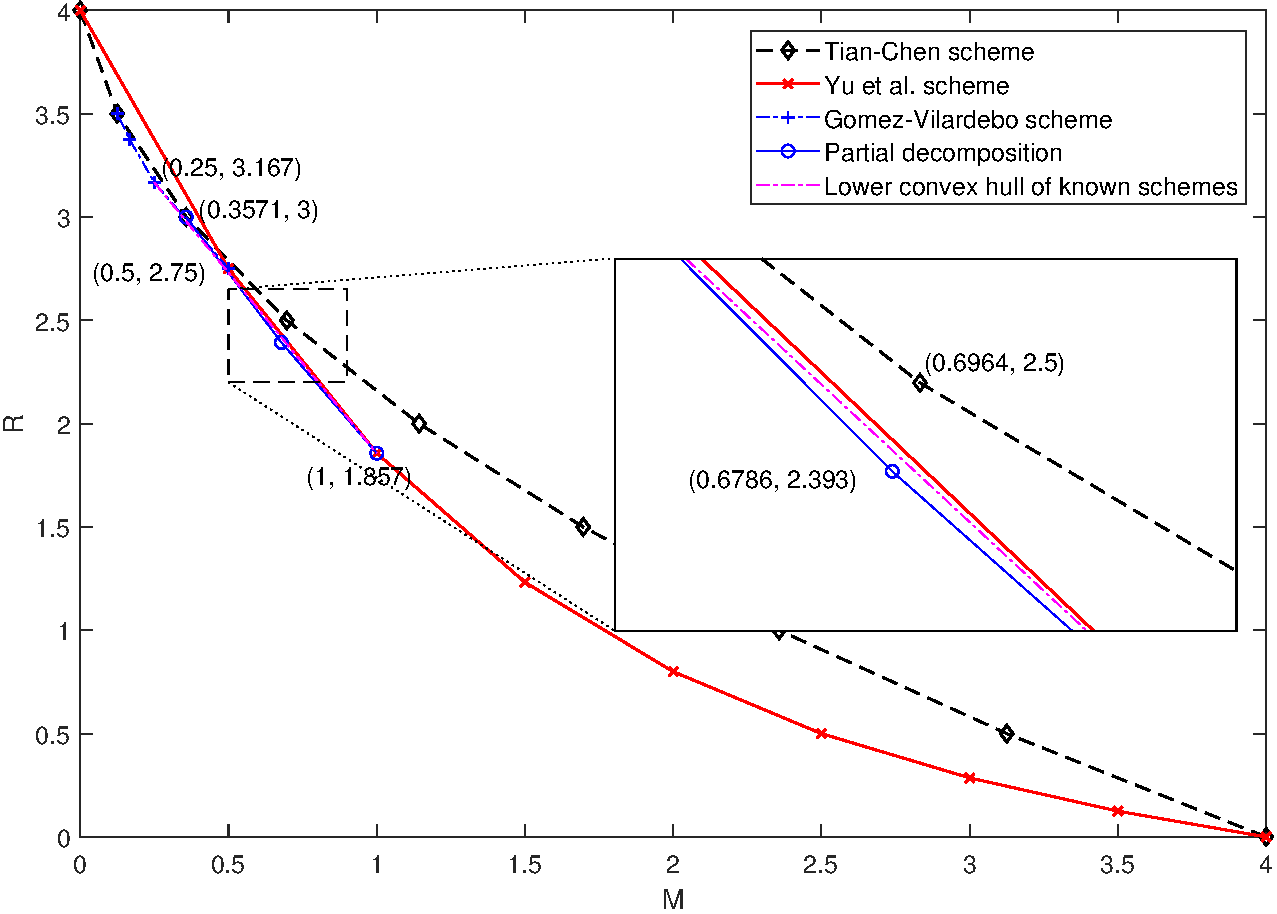
\includegraphics[width=9cm]{N4K8.pdf}\\
{\footnotesize A new information-theoretic inner-bound for caching system $(N,K)=(4,8)$}
\end{figure}
\end{frame}

% ========  13  =================
%\begin{frame}
%\frametitle{A Linear Program}
%\begin{itemize}
%\item Further define 
%\begin{equation*}
%\scalemath{0.9}{
%(M_{\boldsymbol{d}}', R_{\boldsymbol{d}}') =\frac{1}{r\binom{K}{t}} \Bigg( \max_{k \in [1:K]}\sum_{\boldsymbol{\mathcal{P}}_{\boldsymbol{d}}^{(t)}} r_{\boldsymbol{d},\boldsymbol{\mathcal{P}}_{\boldsymbol{d}}^{(t)}} M_{\boldsymbol{d},\boldsymbol{\mathcal{P}}_{\boldsymbol{d}}^{(t)},k}, \sum_{\boldsymbol{\mathcal{P}}_{\boldsymbol{d}}^{(t)}} r_{\boldsymbol{d},\boldsymbol{\mathcal{P}}_{\boldsymbol{d}}^{(t)}} R_{\boldsymbol{d},\boldsymbol{\mathcal{P}}_{\boldsymbol{d}}^{(t)}} \Bigg)
%}
%\end{equation*}
%and 
%\begin{equation*}
%M_r' \triangleq \max_{\boldsymbol{d} \in \mathcal{D}} M_{\boldsymbol{d}}', \qquad R_r' \triangleq \max_{\boldsymbol{d} \in \mathcal{D}} R_{\boldsymbol{d}}' .
%\end{equation*}
%\end{itemize}
%\end{frame}
%
% ========  14  =================
%\begin{frame}
%\frametitle{A Linear Program}
%\begin{itemize}
%\item Choose number of instances $r$ s.t. exist integers $\{r_{\boldsymbol{d},\boldsymbol{\mathcal{P}}_{\boldsymbol{d}}^{(t)}}\}$ 
%\begin{equation*}
%\left|\frac{r_{\boldsymbol{d},\boldsymbol{\mathcal{P}}_{\boldsymbol{d}}^{(t)}}}{r}-\alpha_{\boldsymbol{d},\boldsymbol{\mathcal{P}}_{\boldsymbol{d}}^{(t)}}\right| \leq \epsilon,
%\end{equation*}
%s.t. $\epsilon \geq 0$ and arbitrarily small, we have 
%\begin{equation*}
%\lim_{r \rightarrow \infty}(M_r', R_r')=(M,R)
%\end{equation*}
%be the effective memory-rate pair of the new code.
%\end{itemize}
%\end{frame}

% ========  15  =================
\begin{frame}
\frametitle{Conclusion}
Summary of this work
\begin{itemize}
\item A single scheme unifying two general classes of schemes;
\item Yu scheme and Tian-Chen scheme are two extremes;
\item Transmission type plays an important role;
\item Performance improvement not large: intermediate $M$ regime.% $\rightarrow$ not a surprise.
\end{itemize}

\vspace{0.5cm}
Future work
\begin{itemize}
\item The proposed scheme does not include G{\'o}mez-\\ Vilardeb{\'o}\footnotemark[1]'s scheme: a more generalized code may exist?
\item Simplify linear programming: identify and remove those ``bad" decomposing patterns?
\end{itemize}
\footnotetext[1]{\tiny  J.~G{\'o}mez-Vilardeb{\'o}, ``Fundamental limits of caching: Improved bounds with coded prefetching,'' \emph{arXiv:1612.09071}, Dec. 2016.}
\end{frame}

\end{document}